\documentclass[a4paper,french,10pt]{article}
\usepackage{homework}
\usepackage{diagbox}

% change le nom de la table des matières
\addto\captionsfrench{\renewcommand*\contentsname{Sommaire}}

\lstdefinelanguage{R}%
{morekeywords={function,for,in,if,elseif,else,TRUE,FALSE,%
		return, while, diag, sum, sqrt, nrow, ncol, par, plot, cbind, rep, as, survdiff, survreg, ifelse, anova,
		row, names, colnames, mean, data, frame, model, in, list, rexp, rpois, summary,
		matrix, TRUE, FALSE, for, if, else, function, NA, print, survfit, Surv, rho, ggplot, rnorm},%
	sensitive=true,%
	morecomment=[l]{\#},%
	morestring=[s]{"}{"},%
	morestring=[s]{'}{'},%
}[keywords,comments,strings]%

\lstset{%
	language         = R,
	basicstyle       = \ttfamily,
	keywordstyle     = \bfseries\color{blue},
	stringstyle      = \color{magenta},
	commentstyle     = \color{olive},
	showstringspaces = false,
}

\begin{document}
	
	% Blank out the traditional title page
	\title{\vspace{-1in}} % no title name
	\author{} % no author name
	\date{} % no date listed
	\maketitle % makes this a title page
	
	% Use custom title macro instead
	\usebox{\myReportTitle}
	\vspace{1in} % spacing below title header
	
	% Assignment title
	{\centering \huge \assignmentName \par}
	{\centering \noindent\rule{4in}{0.1pt} \par}
	\vspace{0.05in}
	{\centering \courseCode~: \courseName~ \par}
	{\centering Rédigé le \pubDate\ en \LaTeX \par}
	\vspace{1in}
	
	% Table of Contents
	\tableofcontents
	\newpage
	
	%----------------------------------------------------------------------------------------
	%	EXERCICE 1
	%----------------------------------------------------------------------------------------
	

\section{Introduction}
Le présent projet s'inscrit dans le cadre de l'unité d'enseignement "HAX006X Modèles à variables latentes". L'objectif est ici d'appliquer sur des données réelles, plusieurs méthodes étudiées durant ce cours. Nous nous intéresserons à deux d'entre elles à savoir la méthode par thèmes et  l'algorithme EM (Expectation-Maximization) conçue par Dempster et al., dont l'article est disponible via la source \cite{article}.

\newpage

\section{L'algorithme EM}
Dans cette section nous allons nous intéresser à l'algorithme EM (Expectation-Maximization) afin d'estimer les paramètres $\alpha$, $\mu$ et $\sigma$ d'un mélange gaussien. Nous avons implémenté cet algorithme via la fonction $EM$ (présente dans notre script $R$) en nous aidant de la source \cite{EM_algorithm}. Afin de tester l'efficacité de notre implémentation, nous allons dans un premier temps l'éxecuter sur des données simulées. En effet, dans notre script, nous avons implémenté une autre fonction que nous avons nommé $simulation$. Cette dernière nous permettra de générer de manière aléatoire, un échantillon issu d'un mélange gaussien. Nous décrirons plus en détaille cette fonction, en aval. Dans un second temps, nous exécuterons notre algorithme sur de vraies données afin de voir s'il est robuste. Pour cela nous utiliserons le jeu de données galaxies de la librairie MASS et nous le décrirons ultérieurement.

\subsection{Implémentation de la fonction simulation}
Comme il a été mentionné précédemment nous allons réaliser dans un premier temps une étude sur des données simulées à partir de la fonction $simulation$ (le code de son implémentation est disponible en annexes). Décrivons cette dernière, elle prend en argument:
\begin{itemize}
	\item \textbf{dt\_param:} Le dataframe contenant les paramètres $\alpha$, $\mu$ et $\sigma$
	\item \textbf{n:} La taille de l'échantillon
\end{itemize}
Elle retourne un vecteur de taille $n$ qui sera l'échantillon du mélange gaussien. \\ Regardons un plus en détaille comment a été conçue cette fonction. \\
La partie la plus importante et la plus subtile de ce script est celle dans laquelle nous distribuons aléatoirement les $(X_i)_{i \in 1,\dots,n}$ de l'échantillon de sorte à avoir un bon mélange gaussien. \\
Afin de simplifier les choses, rien de mieux que de prendre un exemple. Dans celui-ci, l'objectif sera de générer un mélange de quatre gaussiennes, ayant pour paramètres respectifs $\theta_1 = (\alpha_1, \mu_1, \sigma_1)$, $\theta_2 = (\alpha_2, \mu_2, \sigma_2)$, $\theta_3 = (\alpha_3, \mu_3, \sigma_3)$ et $\theta_4 = (\alpha_4, \mu_4, \sigma_4)$. \\
Les $(\alpha_j)_{j \in \{1,\dots,4\}}$ étant ici des probabilités, nous avons que:
\[
	\sum_{j=1}^{4} \alpha_{j} = 1
\]
La démarche est la suivante:
\begin{itemize}
	\item On tire $Z \sim \mathcal{U}(0,1)$
	\item Si $Z < \alpha_1$ alors $X \sim \mathcal{N}(\mu_1, \sigma_1)$
	\item Sinon si $\alpha_1 < Z < \alpha_1 + \alpha_2$ alors $X \sim \mathcal{N}(\mu_2, \sigma_2)$
	\item Sinon si $\alpha_1 + \alpha_2 < Z < \alpha_1 + \alpha_2 + \alpha_3$ alors $X \sim \mathcal{N}(\mu_3, \sigma_3)$
	\item Sinon si $\alpha_1 + \alpha_2 + \alpha_3 < Z < \alpha_1 + \alpha_2 + \alpha_3 + \alpha_4$ alors $X \sim \mathcal{N}(\mu_4, \sigma_4)$
\end{itemize}
Notez que notre implémentation marche dans le cas général d'un mélange de J gaussiennes avec $J \in \mathbb{N}^{*}$.

\newpage

\subsection{Implémentation de la fonction EM}
La fonction $EM$ est sans aucun doute celle la plus importante de cette section, il est donc primordial de la décrire (le code de son implémentation est disponible en annexes).\\ 
Tout d'abord, pour implémenter cette dernière, nous nous sommes fortement aidés du pseudo-code suivant:


\begin{algorithm}
	\caption{\textbf{L’algorithme EM (Dempster et al., 1977).}}
	\begin{algorithmic}[1]
		\REQUIRE{$N \in \mathbb{N}$, $\widehat{\theta_0} \in \Theta$, un jeu de données $x_1 \dots x_n$;}
		\ENSURE
		\STATE {$k:=1$;}
		\WHILE {$K < N + 1$}
		\STATE {$\text{\textbf{ETAPE E :} \textit{Calculer la fonction }} Q(\theta;\widehat{\theta}_{k-1}) = \frac{1}{n} \sum_{i=1}^{n} \mathbb{E}_{\widehat{\theta}_{k-1}} [log f(X_i,Z_i,\theta)|X_i = x_i]$;}
		\STATE {$\text{\textbf{ETAPE M : }} \widehat{\theta}_k = argmax \hspace{1.5mm} Q(\theta;\widehat{\theta}_{k-1})$;}
		\STATE {$k \leftarrow k+1$;}
		\ENDWHILE
		\RETURN {$\widehat{\theta}_N$;}
	\end{algorithmic}
\end{algorithm}

La fonction $EM$ prend en argument:
\begin{itemize}
	\item dt\_init, le dataframe contenant les paramètres initiaux ($\alpha_{init}$, $\mu_{init}$, $\sigma_{init}$)
	\item X, les données (réelles ou simulées) issues d'un mélange gaussien
	\item K le nombre d'itérations souhaitées pour l'algorithme
\end{itemize}  
Elle retourne un dataframe contenant les valeurs des
paramètres estimées par l'algorithme, à savoir $\alpha$, $\mu$ et $\sigma$. \\
Les formules que nous avons utilisé pour calculer l'étape E et M et qui sont présentées ci dessous sont issue de la source \cite{EM_algorithm}.
\begin{itemize}
	\item Lors de l'étape E nous déterminons la probabilité $\mathbb{P}_{\tilde{\theta}}(Z = j| X = X_i)$ via la formule suivante:
	\[
	\mathbb{P}_{\tilde{\theta}}(Z = j| X = X_i) = \frac{\alpha_j \times \gamma_{\mu_j, j_v}}{\sum_{k=1}^{J} \alpha_k \times \gamma_{\mu_k, v_k}}
	\] \\
	\item Lors de l'étape M, nous déterminons les estimations des estimateurs du maximum de vraisemblance $(\widehat{\alpha_j}, \widehat{\mu_j}, \widehat{\sigma_j})$ via les formules suivantes:
	\begin{align*}
		\widehat{\alpha_j} &= \displaystyle\frac{1}{n}\sum_{i=1}^n (Z=j|X=X_i) \\
		\widehat{\mu_j} &= \displaystyle\frac{\displaystyle\sum_{i=1}^n X_i (Z=j|X=X_i)}{\displaystyle\sum_{i=1}^n (Z=j|X=X_i)} \\
		\widehat{v_j} &= \displaystyle\frac{\displaystyle\sum_{i=1}^n (X_i -\widehat{\mu_j})^2 (Z=j|X=X_i)}{\displaystyle\sum_{i=1}^n (Z=j|X=X_i)}
	\end{align*} 
\end{itemize}
\vspace{1mm}
Comme en témoigne la section 3.3 (Preuve de la croissance de la vraisemblance d’une itération à l’autre) de la source \cite{EM_algorithm}, il est théoriquement prouvé que l'algorithme permet de faire croître la log-vraisemblance des observations
en les paramètres itérativement créés.
Cependant, il est important de notifier le fait qu'il n'existe pas de convergence de la suite de paramètres établies par l'algorithme EM. En effet, ces derniers peuvent rester bloqués dans des extremas locaux. On comprend donc qu'il est primordial de choisir de bons paramètres initiaux afin de ne pas être confronté à ce problème. Dans la section consacrée à l'étude sur de vraies données, nous expliciterons la procédure qui a été mise en place pour choisir ces paramètres initiaux.

\newpage

\subsection{Étude sur des données simulées}
Cette sous-section sera consacrée à l'étude menée sur des données simulées à partir de notre fonction $simulation$.

\subsubsection{Simulation d'un mélange de deux gaussiennes } 
Nous avons ici décidé de générer un échantillon de taille 100 issu d'un mélange de deux gaussiennes de lois respectives $\mathcal{N}(\mu_1, \sigma_1) = \mathcal{N}(50, 11)$ et $\mathcal{N}(\mu_2, \sigma_2) = \mathcal{N}(220, 50)$.
La densité associée à cet échantillon a été estimée de manière non paramétrique à partir d'une méthode à noyau et elle a été tracée sur la figure \ref{density_sim}.

\begin{figure}[htp] 
	\centering
	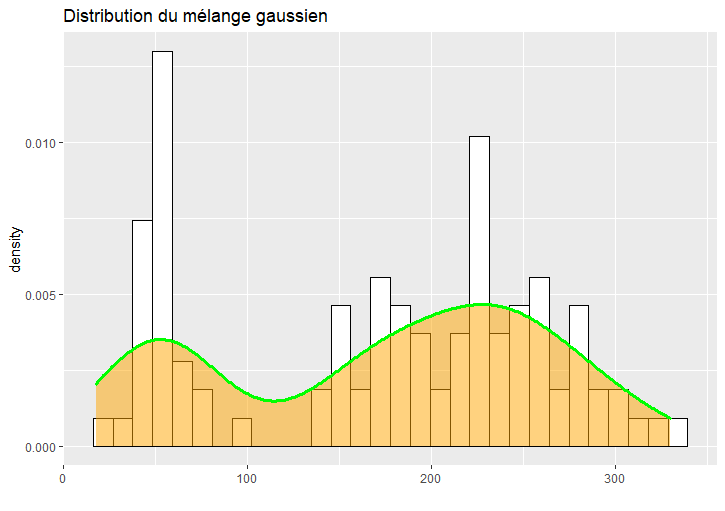
\includegraphics[scale=0.5]{images/dens_sim.png}
	\caption{Densité d'un mélange à 2 gaussiennes estimée par une méthode à noyau}
	\label{density_sim}
\end{figure}

Nous avons ensuite appliqué notre algorithme (fonction EM) sur cet échantillon. Le tableau \ref{tab1} contient les valeurs des vrais paramètres de ce mélange simulé. Comme il a été mentionné précédemment, le choix des paramètres initiaux est crucial si l'on veut que l'algorithme estime correctement les paramètres du mélange. Le tableau \ref{tab2} contient les valeurs des paramètres initiaux utilisés. Comme vous pouvez le voir en observant ces deux tableaux, nous avons choisi des paramètre initiaux assez proches des vrais paramètres (sauf pour la variance du 2ème mélange) de manière à ne pas être bloqué dans des extremas locaux. Les résultats obtenus par notre algorithme sont affichés sur la capture d'écran de la figure \ref{res_sim}.

 Comme on peut le voir sur la figure \ref{res_sim}, les valeurs estimées par notre implémentation sont proches de celles des vrais paramètres (voir tableau \ref{tab1}). Ces résultats nous montrent donc que notre fonction $EM$ fonctionne correctement, ce qui est rassurant.
 
 \begin{table}[htp]
 	\center
 	\begin{tabular}{|c||c|c|c|}
 		\hline
 		& $\alpha$ & $\mu$ & $\sigma$\\
 		\hline
 		Paramètres du 1er mélange & $0.4$ & $50$ & $11$ \\
 		\hline
 		Paramètres du 2ème mélange & $0.6$ & $220$ & $50$ \\
 		\hline
 	\end{tabular}
 	\caption{Vrais paramètres du mélange}
 	\label{tab1}
 \end{table}

\begin{table}[htp]
	\center
	\begin{tabular}{|c||c|c|c|}
		\hline
		& $\alpha_{init}$ & $\mu_{init}$ & $\sigma_{init}$\\
		\hline
		Paramètres du 1er mélange & $0.2$ & $30$ & $21$ \\
		\hline
		Paramètres du 2ème mélange & $0.8$ & $280$ & $160$ \\
		\hline
	\end{tabular}
	\caption{Paramètres initiaux}
	\label{tab2}
\end{table}
 
 \begin{figure}[htp] 
 	\centering
 	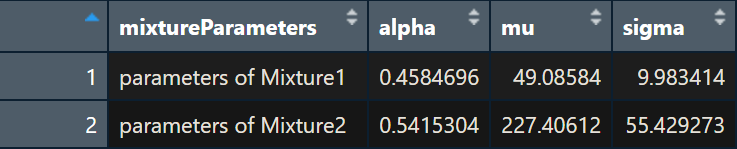
\includegraphics[scale=0.9]{images/res_sim.png}
 	\caption{Paramètres du mélange gaussien estimés par notre fonction $EM$}
 	\label{res_sim}
 \end{figure}

\newpage


\subsubsection{Simulation d'un mélange à quatre gaussiennes}
Nous avons ici décidé de générer un échantillon de taille 1000 issu d'un mélange de quatre gaussiennes de lois respectives:
\begin{itemize}
	\item $\mathcal{N}(\mu_1, \sigma_1) = \mathcal{N}(35, 11)$
	\item $\mathcal{N}(\mu_2, \sigma_2) = \mathcal{N}(350, 22)$
	\item $\mathcal{N}(\mu_3, \sigma_3) = \mathcal{N}(720, 32)$
	\item $\mathcal{N}(\mu_4, \sigma_4) = \mathcal{N}(1198, 55)$
\end{itemize}
La densité associée à cet échantillon a été estimée de manière non paramétrique à partir d'une méthode à noyau et elle a été tracée sur la figure \ref{density_sim2}.

\begin{figure}[htp] 
	\centering
	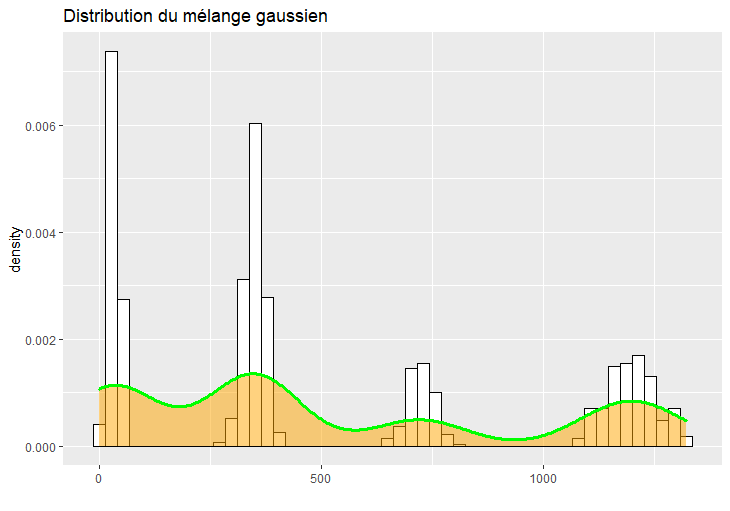
\includegraphics[scale=0.5]{images/dens_sim2.png}
	\caption{Densité d'un mélange à 4 gaussiennes estimée par une méthode à noyau}
	\label{density_sim2}
\end{figure}

Nous avons ensuite appliqué notre algorithme (fonction EM) sur cet échantillon. Le tableau \ref{tab3} contient les valeurs des vrais paramètres de ce mélange simulé. Comme il a été mentionné précédemment, le choix des paramètres initiaux est crucial si l'on veut que l'algorithme estime correctement les paramètres du mélange. Le tableau \ref{tab4} contient les valeurs des paramètres initiaux utilisés. Comme vous pouvez le voir en observant ces deux tableaux, nous avons choisi des paramètre initiaux assez proches des vrais de manière à ne pas être bloqué dans des extremas locaux. Les résultats obtenus par notre algorithme sont affichés sur la capture d'écran de la figure \ref{res_sim2}.

Comme on peut le voir sur la figure \ref{res_sim2}, les valeurs estimées par notre implémentation sont proches de celles des vrais paramètres (voir tableau \ref{tab3}). Ces résultats nous confortent une fois de plus dans l'idée que notre fonction $EM$ fonctionne correctement.

\begin{table}[htp]
	\center
	\begin{tabular}{|c||c|c|c|}
		\hline
		& $\alpha$ & $\mu$ & $\sigma$\\
		\hline
		Paramètres du 1er mélange & $0.30$ & $35$ & $11$ \\
		\hline
		Paramètres du 2ème mélange & $0.33$ & $350$ & $22$ \\
		\hline
		Paramètres du 3ème mélange & $0.15$ & $720$ & $32$ \\
		\hline
		Paramètres du 4ème mélange & $0.22$ & $1198$ & $55$ \\
		\hline
	\end{tabular}
	\caption{Vrais paramètres du mélange}
	\label{tab3}
\end{table}

\begin{table}[htp]
	\center
	\begin{tabular}{|c||c|c|c|}
		\hline
		& $\alpha$ & $\mu$ & $\sigma$\\
		\hline
		Paramètres du 1er mélange & $0.33$ & $30$ & $10$ \\
		\hline
		Paramètres du 2ème mélange & $0.30$ & $370$ & $25$ \\
		\hline
		Paramètres du 3ème mélange & $0.17$ & $717$ & $30$ \\
		\hline
		Paramètres du 4ème mélange & $0.20$ & $1238$ & $57$ \\
		\hline
	\end{tabular}
	\caption{Paramètres initiaux choisis}
	\label{tab4}
\end{table}

\begin{figure}[htp] 
	\centering
	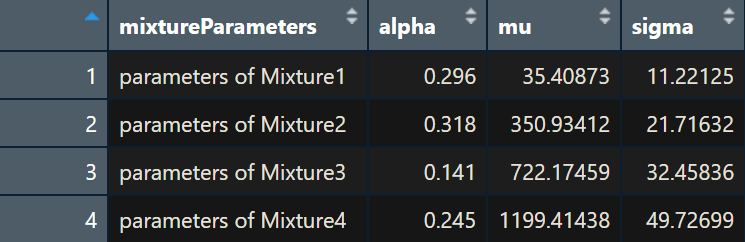
\includegraphics[scale=0.8]{images/res_sim2.png}
	\caption{Paramètres du mélange gaussien estimés par notre fonction $EM$}
	\label{res_sim2}
\end{figure}


%\begin{figure}[htp] 
%	\centering
%	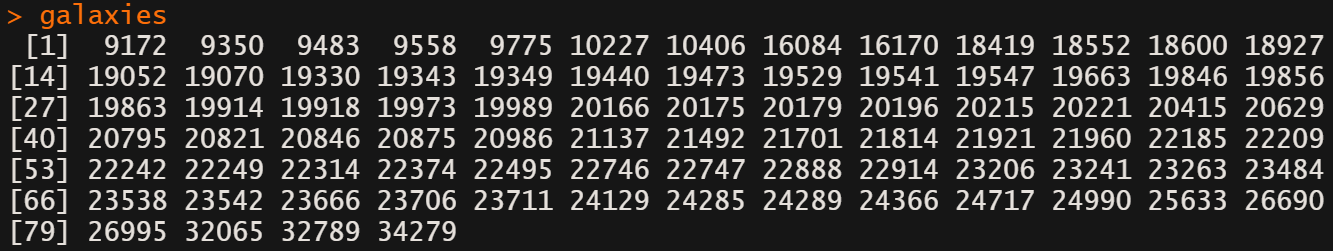
\includegraphics[scale=0.45]{images/dataset.png}
%	\caption{Extrait du jeu de données $galaxies$}
%	\label{galaxies}
%\end{figure}


\subsection{Comparaison de la fonction $EM$ avec $mixtools$ sur des données réelles}
Dans cette section, l'étude sera menée sur des données réelles. Nous utiliserons le jeu de données $galaxies$ provenant de la librairie $MASS$ de $R$. Dans un premier temps, nous allons estimer les paramètres du mélange associés à ce dataset via l'utilisation de notre implémentation de l'algorithme EM (la fonction EM). Nous estimerons ensuite une seconde fois les paramètres de ce même mélange mais cette fois-ci, en utilisant la fonction $normalmixEM$ prédéfinie de $R$ qui est disponible via le package $mixtools$. Nous avons choisi d'utiliser cette librairie car l'algorithme EM y est implémenté et il est utilisé par la fonction $normalmixEM$ pour estimer les paramètres d'un mélange. Le fait de comparer les résultats de notre fonction avec ceux obtenus par celle prédéfini de $R$ nous permettra d'évaluer la performance et la robustesse de notre implémentation sur de vraies données.\\
Le jeu de données $Galaxies$ est un vecteur numérique qui représente les vitesses en km/s (kilomètres par secondes) de $82$ galaxies. La figure \ref{galaxies} est un extrait de ce jeu de données.

\begin{figure}[htp] 
	\centering
	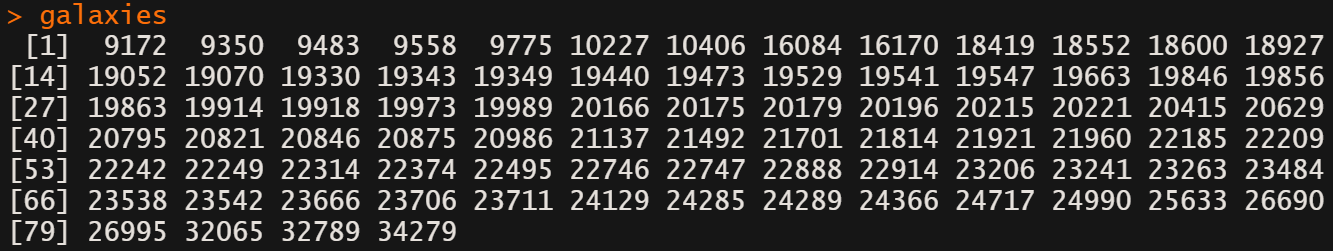
\includegraphics[scale=0.7]{images/dataset.png}
	\caption{Extrait du jeu de données $galaxies$}
	\label{galaxies}
\end{figure}

Comme il a été mentionné dans la section 2.2, si l'on veut obtenir de bonnes estimations pour les paramètres du mélange, il est primordial de sélectionner correctement les paramètres qui serviront de conditions initiales pour l'algorithme. Nous allons donc détailler la stratégie qui a été mise en place pour sélectionner ces derniers. Étant donné que nous ne connaissons pas la vraie densité associée à ces données, nous avons utilisé dans un premier temps une méthode d'estimation non paramétrique (à noyau) afin de d'estimer cette dernière. La figure \ref{realDataDensEst} représente la courbe de densité estimée par la méthode à noyau. 

\newpage

\begin{figure}[htp] 
	\centering
	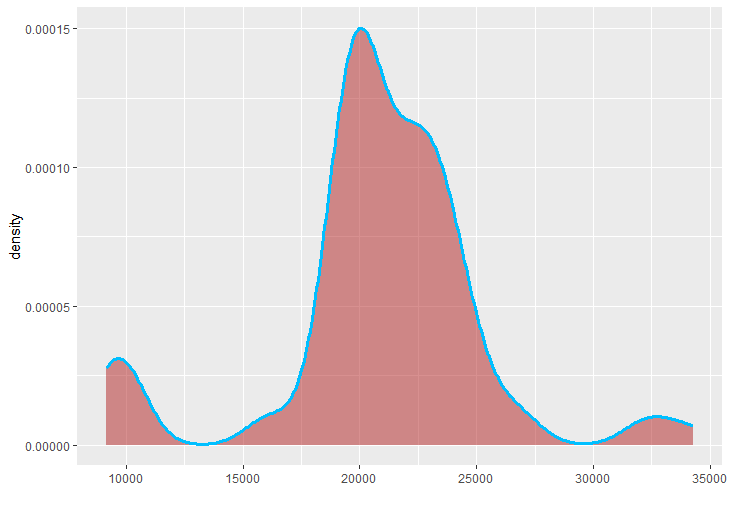
\includegraphics[scale=0.5]{images/realDataDensEst.png}
	\caption{Densité du dataset $galaxies$ estimée par une méthode à noyau}
	\label{realDataDensEst}
\end{figure}

En observant la figure \ref{realDataDensEst}, on peut facilement distinguer 3 pics principaux. Un premier vers 9800 sur l'axe des abscisses, un deuxième vers 21000 et un 3ème vers 32000. Il semblerait aussi y avoir une sorte de pic vers 24000 mais celui-ci n'étant pas clairement visible nous ne le considérerons pas. On supposera donc pour la suite de l'étude que nous somme dans le cas d'un mélange à 3 composantes. \\
Il nous faudra donc déterminer les paramètres:
\begin{itemize}
	\item $\alpha_1$,$\alpha_2$ et $\alpha_3$ qui sont les proportions associées aux 3 gaussiennes
	\item $\mu_1$,$\mu_2$ et $\mu_3$ qui sont les moyennes des 3 gaussiennes
	\item $\sigma_1$,$\sigma_2$ et $\sigma_3$ qui sont les ecart-types des 3 gaussiennes
\end{itemize}
Pour commencer, nous dirons que les paramètres $(\alpha_{j})_{j \in \{1,\dots3\}}$ qui seront utilisés dans les conditions initiale seront tous égaux, c'est à dire que $(\alpha_1)_{init} = (\alpha_2)_{init} = (\alpha_3)_{init} = \frac{1}{3}$ (car il faut que $\sum_{i=1}^{3} \alpha_j = 1$).

\vspace{2mm}

Pour la recherche des paramètres $(\mu_j)_{j \in \{1,\dots,3\}}$ et $(\sigma_j)_{j \in \{1, \dots, 3\}}$ initiaux, nous allons nous aider de la figure \ref{extremumLoc}.

\begin{figure}[htp] 
	\centering
	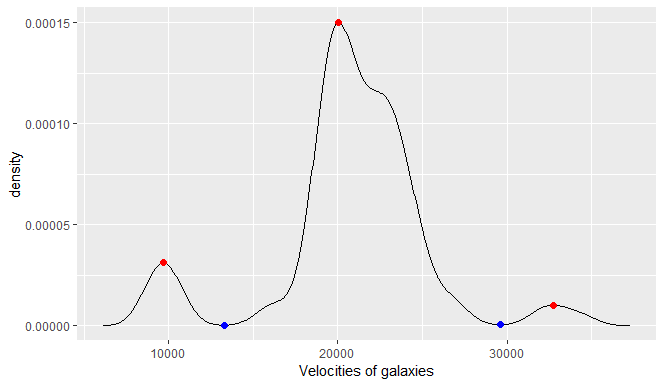
\includegraphics[scale=0.6]{images/extremumLoc.png}
	\caption{Extremums locaux de la densité estimée du dataset $galaxies$}
	\label{extremumLoc}
\end{figure}

À l'aide de la fonction $find\_peaks()$ du package $ggpmisc$ et de la fonction $local.min.max()$ du package $spatialEco$, nous avons pu déterminer les extremums locaux de la courbe de densité estimée des données $galaxies$. Les maximums locaux sont représentés par les points rouges et les minimums locaux par les points bleus sur la figure \ref{extremumLoc}.

\newpage

Les paramètres $(\mu_j)_{j \in \{1,\dots,3\}}$ qui seront utilisés dans les conditions initiales seront donc les abscisses respectives de ces 3 maximums locaux. Nous aurons donc:
\begin{itemize}
	\item $(\mu_1)_{init} = 9698.471$
	\item $(\mu_2)_{init} = 20050.850$
	\item $(\mu_3)_{init} = 32717.292$
\end{itemize}

\vspace{2mm}

Les $(\alpha_j)_{j \in \{1,\dots,3\}}$ et les $(\mu_j)_{j \in \{1,\dots,3\}}$ initiaux ayant été déterminés, il ne nous reste plus qu'à trouver les $(\sigma_j)_{j \in \{1,\dots,3\}}$ initiaux. Nous allons les déterminer en calculant les écarts-types de chacun des 3 piques. Tout d'abord, nous scindons nos données en 3 intervalles car il y a 3 piques. C'est à ce moment là qu'interviennent les minimas locaux. En effet, c'est eux qui vont justement nous permettre de délimiter notre jeu de données en 3 intervalles. \\
Le premier intervalle sera composé des abscisses allant du début du jeu de données jusqu'à l'abscisse du premier minimum local. Le deuxième intervalle quant à lui sera composé des valeurs des abscisses allant du premier minimum local jusqu'au deuxième minimum local. Enfin le dernier intervalle contiendra les abscisses allant du deuxième minimum local jusqu'a la fin du jeu de données. Dans la liste à puces ci-dessous nous avons expliciter les bornes $inf$ et $sup$ de chacun des trois intervalles:
\begin{itemize}
	\item \textbf{Première intervalle:} $[6166.482; 13291.36]$
	\item \textbf{Deuxième intervalle:} $[13291.36; 29611.58]$
	\item \textbf{Troisième intervalle:} $[29611.58; 37284.52]$
\end{itemize}
En appliquant la fonction $sd()$ sur le premier intervalle nous obtiendrons $(\sigma_1)_{init}$. En appliquant la fonction $sd()$ sur le deuxième intervalle nous obtiendrons $(\sigma_2)_{init}$. Nous procéderons de même pour avoir $(\sigma_3)_{init}$. Au final, nous obtenons que:
\begin{itemize}
	\item $(\sigma_1)_{init} = 2083.124$
	\item $(\sigma_2)_{init} = 4737.603$
	\item $(\sigma_3)_{init} = 2241.339$
\end{itemize}
L'ensemble des paramètres initiaux qui ont été déterminés précédemment sont résumés dans le tableau \ref{tab5}.

\begin{table}[htp]
	\center
	\begin{tabular}{|c||c|c|c|}
		\hline
		& $\alpha_{init}$ & $\mu_{init}$ & $\sigma_{init}$\\
		\hline
		Paramètres du 1er mélange & $\frac{1}{3}$ & $9698.471$ & $2083.124$ \\
		\hline
		Paramètres du 2ème mélange & $\frac{1}{3}$ & $20050.850$ & $4737.603$ \\
		\hline
		Paramètres du 3ème mélange & $\frac{1}{3}$ & $32717.292$ & $2241.339$ \\
		\hline
	\end{tabular}
	\caption{Paramètres initiaux}
	\label{tab5}
\end{table}

Maintenant que nous avons toutes nos conditions initiales, nous sommes en mesure d'exécuter notre implémentation de l'algorithme $EM$ sur les vraies données $galaxies$. Les paramètres du mélange estimés par notre fonction $EM$ sont visibles sur la capture d'écran (figure \ref{res_EM}). Nous les avons également résumé dans le tableau \ref{tab6} pour une meilleur visibilité. 

\begin{figure}[htp] 
	\centering
	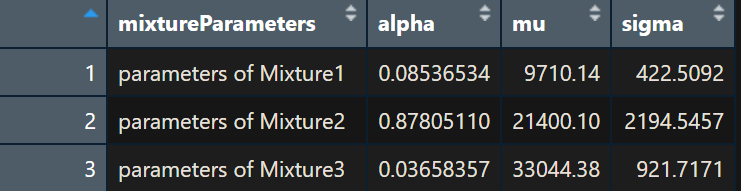
\includegraphics[scale=0.8]{images/paramEstEM.png}
	\caption{Paramètres estimées par notre fonction $EM$}
	\label{res_EM}
\end{figure}

\begin{table}[htp]
	\center
	\begin{tabular}{|c||c|c|c|}
		\hline
		& $\alpha$ & $\mu$ & $\sigma$\\
		\hline
		Paramètres du 1er mélange estimés par $EM$ & $0.08536534$ & $9710.14$ & $422.5092$ \\
		\hline
		Paramètres du 2ème mélange estimés par $EM$ & $0.87805110$ & $21400.10$ & $2194.5457$ \\
		\hline
		Paramètres du 3ème mélange estimés par $EM$ & $0.03658357$ & $33044.38$ & $921.7171$ \\
		\hline
	\end{tabular}
	\caption{Paramètres estimées par notre fonction $EM$}
	\label{tab6}
\end{table}

\newpage

Maintenant que nous avons les paramètres du mélange, estimés par notre implémentation, comparons les avec ceux obtenus en utilisant la fonction $normalmixEM$ de $R$ dans laquelle est implémenté l'algorithme EM. La figure \ref{paramEstLib} est une capture d'écran dans laquelle sont stockés tous les paramètres estimés par la fonction $normalmixEM$ de $R$. Nous les avons également résumé dans le tableau \ref{tab7} pour une meilleur visibilité.  

\begin{figure}[htp] 
	\centering
	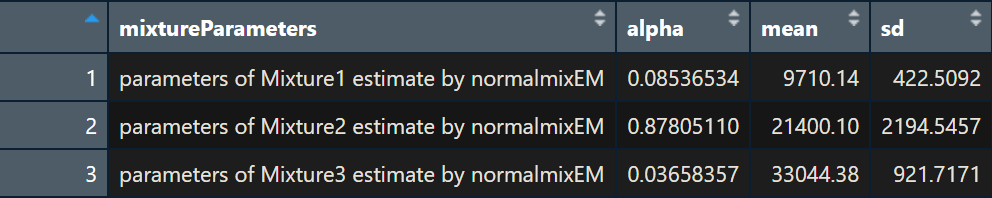
\includegraphics[scale=0.8]{images/paramEstLib.png}
	\caption{Paramètres estimées par $normalmixEM$}
	\label{paramEstLib}
\end{figure}

\begin{table}[htp]
	\center
	\begin{tabular}{|c||c|c|c|}
		\hline
		& $\alpha$ & $\mu$ & $\sigma$\\
		\hline
		Paramètres du 1er mélange estimés par $normalmixEM$ & $0.08536534$ & $9710.14$ & $422.5092$ \\
		\hline
		Paramètres du 2ème mélange estimés par $normalmixEM$ & $0.87805110$ & $21400.10$ & $2194.5457$ \\
		\hline
		Paramètres du 3ème mélange estimés par $normalmixEM$ & $0.03658357$ & $33044.38$ & $921.7171$ \\
		\hline
	\end{tabular}
	\caption{Paramètres estimées par notre fonction $EM$}
	\label{tab7}
\end{table}

En regardant les tableaux \ref{tab6} et \ref{tab7}, on constate que les valeurs des paramètres estimées avec notre fonction $EM$ et celles estimées avec la fonction $normalmixEM$ sont exactement les mêmes. Cela nous montre donc que notre implémentation de l'algorithme EM est robuste et qu'elle peut être aussi utilisée sur des données réelles de mélanges. Notre fonction $EM$ fournira donc de bonnes estimations aussi bien sur des données simulées que sur des données réelles à partir du moment où les conditions initiales sont correctement choisies.

%\begin{figure}[htp] 
%	\centering
%	\subfloat[seuil $\approx 2.7$]{%
%		\includegraphics[scale=0.4]{images/sumBadth.png}%
%	}%
%	\hfill%
%	\subfloat[seuil $\approx 3.65$]{%
%		\includegraphics[scale=0.4]{images/sumGoodth.png}%
%	}%
%	\caption{Résultats donnés en sortie de la fonction \textit{fpot} pour les 2 seuils}
%	\label{summary}
%\end{figure}


%\begin{table}[htp]
%	\center
%	\begin{tabular}{|c||c|c|c|}
%		\hline
%		\diagbox{Niveau de retour}{Périodes ou Années $T$} & $T = 100$ & $T = 500$ & $T = 1000$\\
%		\hline
%		$x_{\frac{1}{T}}$ & $4.686475$ & $4.72502$ & $4.723653$ \\
%		\hline
%	\end{tabular}
%	\caption{Niveaux de retour associés aux périodes de retour $T$}
%	\label{tab3}
%\end{table}

\newpage

\section{Conclusion}

À vues des résultats et des comparaisons faites entre notre fonction $EM$ et celle $normalmixEM$ du package $mixtools$, nous pouvons conclure que notre implémentation fournira de bonnes estimations aussi bien sur des données simulées que sur des données réelles de mélanges à condition bien évidemment de choisir correctement les conditions initiales. Une piste d'amélioration possible de notre fonction serait d'y ajouter une fonctionnalité de recherche automatique de paramètres initiaux. D'après la littérature, plusieurs techniques peuvent être envisagées. Parmi celles qui reviennent le plus souvent on retrouve la méthode des kmeans ou celle des recuits.


\newpage

\section{Annexes}
\subsection{Script de la fonction $simulation$}
Ci dessous, l'export de code de la fonction $simulation$.
\lstinputlisting[language=R, firstline=15, lastline=41]{code/scriptProject_COME_PRALON.R}

\newpage

\subsection{Script de la fonction $EM$}
Ci dessous, l'export de code de la fonction $EM$.
\lstinputlisting[language=R, firstline=76, lastline=123]{code/scriptProject_COME_PRALON.R}

\newpage

\subsection{Script de la fonction $plot\_distrib$}
Ci dessous, l'export de code de la fonction $plot\_distrib$. \\
Cette fonction permet d'afficher l'histogramme des données ainsi que la courbe de densité estimée associée à ces données. Cette courbe de densité sera superposée à l'histogramme.
\lstinputlisting[language=R, firstline=46, lastline=52]{code/scriptProject_COME_PRALON.R}

\newpage

\section{Bibliographie}

\renewcommand\refname{}
\begin{thebibliography}{9}
	\bibitem{article}
	Dempster A.P., Laird N. M., Rubin D. B. (1977). Maximum Likelihood from Incomplete Data via the EM Algorithm, Journal of the Royal Statistical Society, Series B, Vol. 39, 1, 1-38
	\bibitem{EM_algorithm}
	Frédéric Santos (2015). L'algorithme EM : une courte présentation
	\url{https://members.loria.fr/moberger/Enseignement/AVR/Exposes/algo-em.pdf}
\end{thebibliography}

\end{document}
